\batchmode
\documentclass[a4paper,11pt]{cernman}
\usepackage{html,example,rotating,texnames}

 


















 
%




























%

























\begin{latexonly}
\makeindex
\hoffset=0mm
\end{latexonly}


\def\fileversion{v4.0}

\def\filedate{95/08/03}

\def\docdate{95/08/03}

\newcommand {\Larg}[1]{{\rmfamily\itshape\mdseries #1\/}}

\newcommand {\Largb}[1]{\lcb{\rmfamily\itshape\mdseries #1\/}\rcb}

\newcommand {\Largs}[1]{\lsb{\rmfamily\itshape\mdseries #1\/}\rsb}

\newcommand {\DefC}[1]{\Lcs{#1}}

\newcommand {\DefCm}[2]{\Lcs{#1}\Largb{#2}}

\newcommand {\DefCo}[2]{\Lcs{#1}\Largb{#2}}

\newcommand {\DefCmo}[3]{\Lcs{#1}\Largb{#2}\Largs{#3}}

\newcommand {\DefCom}[3]{\Lcs{#1}\Largs{#2}\Largb{#3}}

\newcommand {\DefCmm}[3]{\Lcs{#1}\Largb{#2}\Largb{#3}}

\newcommand {\DefComm}[4]{\Lcs{#1}\Largs{#2}\Largb{#3}\Largb{#4}}

\newcommand {\DefCmmm}[4]{\Lcs{#1}\Largb{#2}\Largb{#3}\Largb{#4}}

\newcommand {\DefCmmmm}[5]{\Lcs{#1}\Largb{#2}\Largb{#3}\Largb{#4}\Largb{#5}}

\newcommand {\DefCommm}[5]{\Lcs{#1}\Largs{#2}\Largb{#3}\Largb{#4}\Largb{#5}}

\newcommand {\DefCmmmmm}[6]{\Lcs{#1}\Largb{#2}\Largb{#3}\Largb{#4}\Largb{#5}\Largb{#6}}

\newcommand {\DefCommmm}[6]{\Lcs{#1}\Largs{#2}\Largb{#3}\Largb{#4}\Largb{#5}\Largb{#6}}

\newenvironment {BCmd}{\flushleft}{\endflushleft}

\newcommand {\BDefC}[1]{\begin{BCmd}\fbox{\DefC{#1}}\end{BCmd}}

\newcommand {\BDefCm}[2]{\begin{BCmd}\fbox{\DefCm{#1}{#2}}\end{BCmd}}

\newcommand {\BDefCo}[2]{\begin{BCmd}\fbox{\DefCo{#1}{#2}}\end{BCmd}}

\newcommand {\BDefCmo}[3]{\begin{BCmd}\fbox{\DefCmo{#1}{#2}{#3}}\end{BCmd}}

\newcommand {\BDefCom}[3]{\begin{BCmd}\fbox{\DefCom{#1}{#2}{#3}}\end{BCmd}}

\newcommand {\BDefCmm}[3]{\begin{BCmd}\fbox{\DefCmm{#1}{#2}{#3}}\end{BCmd}}

\newcommand {\BDefComm}[4]{\begin{BCmd}\fbox{\DefComm{#1}{#2}{#3}{#4}}\end{BCmd}}

\newcommand {\BDefCmmm}[4]{\begin{BCmd}\fbox{\DefCmmm{#1}{#2}{#3}{#4}}\end{BCmd}}

\newcommand {\BDefCmmmm}[5]{\begin{BCmd}\fbox{\DefCmmmm{#1}{#2}{#3}{#4}{#5}}\end{BCmd}}

\newcommand {\BDefCommm}[5]{\begin{BCmd}\fbox{\DefCommm{#1}{#2}{#3}{#4}{#5}}\end{BCmd}}

\newcommand {\BDefCmmmmm}[6]{\begin{BCmd}\fbox{\DefCmmmmm{#1}{#2}{#3}{#4}{#5}{#6}}\end{BCmd}}

\newcommand {\BDefCommmm}[6]{\begin{BCmd}\fbox{\DefCommmm{#1}{#2}{#3}{#4}{#5}{#6}}\end{BCmd}}

\renewcommand {\Lenv}[1]{\mbox{\texttt{#1}}{\index{#1@{\tt #1} environment}}}

\newcommand {\LBEG}[1]{{\rm\tt\bs{}begin\lcb #1\rcb}{\index{#1@{\tt #1} environment}}}

\newcommand {\LEND}[1]{{\rm\tt\bs{}end\lcb #1\rcb}{\index{#1@{\tt #1} environment}}}

\newcommand {\DefE}[1]{\LBEG{#1}}

\newcommand {\DefEm}[2]{\LBEG{#1}\Largb{#2}}

\newcommand {\DefEo}[2]{\LBEG{#1}\Largs{#2}}

\newcommand {\DefEmo}[3]{\LBEG{#1}\Largb{#2}\Largs{#3}}

\newcommand {\DefEom}[3]{\LBEG{#1}\Largs{#2}\Largb{#3}}

\newcommand {\DefEmm}[3]{\LBEG{#1}\Largb{#2}\Largb{#3}}

\newcommand {\DefEmom}[4]{\LBEG{#1}\Largb{#2}\Largs{#3}\Largb{#4}}

\newcommand {\DefEomm}[4]{\LBEG{#1}\Largs{#2}\Largb{#3}\Largb{#4}}

\newcommand {\DefEmoo}[4]{\LBEG{#1}\Largb{#2}\Largs{#3}\Largs{#4}}

\newcommand {\DefEomo}[4]{\LBEG{#1}\Largs{#2}\Largb{#3}\Largs{#4}}

\newcommand {\DefEmmm}[4]{\LBEG{#1}\Largb{#2}\Largb{#3}\Largb{#4}}

\newcommand {\BDefE}[1]{\begin{BCmd}\fbox{\DefE{#1}}\end{BCmd}}

\newcommand {\BDefEm}[2]{\begin{BCmd}\fbox{\DefEm{#1}{#2}}\end{BCmd}}

\newcommand {\BDefEo}[2]{\begin{BCmd}\fbox{\DefEo{#1}{#2}}\end{BCmd}}

\newcommand {\BDefEmo}[3]{\begin{BCmd}\fbox{\DefEmo{#1}{#2}{#3}}\end{BCmd}}

\newcommand {\BDefEom}[3]{\begin{BCmd}\fbox{\DefEom{#1}{#2}{#3}}\end{BCmd}}

\newcommand {\BDefEmm}[3]{\begin{BCmd}\fbox{\DefEmm{#1}{#2}{#3}}\end{BCmd}}

\newcommand {\BDefEmom}[4]{\begin{BCmd}\fbox{\DefEmom{#1}{#2}{#3}{#4}}\end{BCmd}}

\newcommand {\BDefEomm}[4]{\begin{BCmd}\fbox{\DefEomm{#1}{#2}{#3}{#4}}\end{BCmd}}

\newcommand {\BDefEmoo}[4]{\begin{BCmd}\fbox{\DefEmoo{#1}{#2}{#3}{#4}}\end{BCmd}}

\newcommand {\BDefEomo}[4]{\begin{BCmd}\fbox{\DefEomo{#1}{#2}{#3}{#4}}\end{BCmd}}

\newcommand {\BDefEmmm}[4]{\begin{BCmd}\fbox{\DefEmmm{#1}{#2}{#3}{#4}}\end{BCmd}}

\newcommand {\LMsty}[1]{\texttt{#1}\index{#1@{\texttt{#1} style}}}

\def\Lmsty#1{\LMsty{#1}}

\def\vref#1{\ref{#1}}

\renewcommand {\DVI}{\texttt{dvi}\index{dvi file}}

\newcommand {\DVIPS}{\texttt{dvips}\index{dvips program}}

\newcommand {\gif}{gif\index{gif}}

\newcommand {\Html}{HTML\index{HTML}}

\renewcommand {\PS}{PostScript\index{PostScript}}

\newcommand {\PTD}{\texttt{ptd}\index{ptd program}}

\newcommand {\SGML}{SGML\index{SGML}}

\newcommand {\URL}{URL\index{URL!Universal Resource Locator}}

\def\X#1{#1 &\tt\string#1}

\newcommand {\UkeV}{\mbox{kev}}

\newcommand {\UMeV}{\mbox{Mev}}

\newcommand {\UGeV}{\mbox{Gev}}

\newcommand {\UTeV}{\mbox{Tev}}

\newcommand {\Pe}{\mbox{$\mathrm{e}$}}

\newcommand {\Pme}{\mbox{$m_{\mathrm{e}}$}}

\newcommand {\Pem}{\mbox{$\mathrm{e}^-$}}

\newcommand {\Pep}{\mbox{$\mathrm{e}^+$}}

\def\X#1{#1 &\tt\string #1}

\makeatother
\newenvironment{tex2html_wrap}{}{}
\newwrite\lthtmlwrite
\def\lthtmltypeout#1{{\let\protect\string\immediate\write\lthtmlwrite{#1}}}%
\newbox\sizebox
\begin{document}
\pagestyle{empty}
\setcounter{page}{2}
\setcounter{page}{1}
\stepcounter{chapter}
\stepcounter{section}
\stepcounter{section}
\stepcounter{section}
\stepcounter{subsection}
\stepcounter{chapter}
\stepcounter{section}
{\newpage
\clearpage
\samepage \fbox{\Lcs{Sxxx}\lsb{\rmfamily\itshape\mdseries margintext\/}\rsb\lcb{\rmfamily\itshape\mdseries labeltext\/}\rcb\lcb{\rmfamily\itshape\mdseries maintext\/}\rcb\lcb{\rmfamily\itshape\mdseries parameters\/}\rcb}
}

\stepcounter{section}
{\newpage
\clearpage
\samepage \begin{tabular}{@{}ll}
\multicolumn{1}{c}{\bf Environment} & \multicolumn{1}{c}{\bf Description} \\ 
\DefEm{DL}{width}                   & Description list with width of 
                                      largest item                        \\ 
                                    & Text of term is in bold             \\ 
\DefEm{DLtt}{width}                 & Description list with width of 
                                      largest item                        \\ 
                                    & Text of term is in teletype font    \\ 
\DefEm{DLc}{width}                  & Denser version of \mbox{\texttt{DL}}{\index{DL@{\tt DL} environment}} list    \\ 
\DefEm{DLctt}{width}                & Denser version of \mbox{\texttt{DLtt}}{\index{DLtt@{\tt DLtt} environment}} list  \\ 
\DefE{OL}                           & Numbered (ordered) list             \\ 
\DefE{OLc}                          & Dense numbered (ordered) list       \\ 
\DefE{UL}                           & Unnumbered (itemize) list           \\ 
\DefE{ULc}                          & Dense unnumbered (itemize) list     \\ 
\end{tabular}
}

{\newpage
\clearpage
\samepage \begin{example}\begin{DLtt}{12345}
  \item[CHOPT] Option chosen
  \item[ID]    Identifier
  \item[IFLAG] Flag
    \begin{DLtt}{1}
      \item[0] Start
      \item[1] Continue
      \item[2] Stop
    \end{DLtt}
\end{DLtt}
\end{example}
}

\stepcounter{section}
{\newpage
\clearpage
\samepage \fbox{\begin{tabular}{@{}l}%
  \DefE{XMP}\\ 
  \DefEm{XMPt}{Example title}
      \end{tabular}}
}

{\newpage
\clearpage
\samepage \begin{example}\par\begin{XMP}\end{XMP}
\end{example}
}

\stepcounter{chapter}
{\newpage
\clearpage
\samepage \begin{Tabhere}% latex2html id marker 633
\begin{center}
\begin{tabular}{*{10}{l}}
\ &\tt\string \amp   &\ &\tt\string \apos    &\ &\tt\string \Ast      &\ &\tt\string \atsign &\ &\tt\string \bs     \\ 
\ &\tt\string \bsol  &\ &\tt\string \Circ    &\ &\tt\string \Colon    &\ &\tt\string \commat &\ &\tt\string \dollar \\ 
\ &\tt\string \excl  &\ &\tt\string \hyphen  &\ &\tt\string \lab      &\ &\tt\string \lcb    &\ &\tt\string \lcub   \\ 
\ &\tt\string \lpar  &\ &\tt\string \lsb     &\ &\tt\string \lsqb     &\ &\tt\string \lsquo  &\ &\tt\string \num    \\ 
\ &\tt\string \period&\ &\tt\string \percent &\ &\tt\string \percnt   &\ &\tt\string \quest  &\ &\tt\string \quot   \\ 
\ &\tt\string \rab   &\ &\tt\string \rcb     &\ &\tt\string \rcub     &\ &\tt\string \rpar   &\ &\tt\string \rsb    \\ 
\ &\tt\string \rsqb  &\ &\tt\string \rsquo   &\ &\tt\string \sbl      &\ &\tt\string \semi   &\ &\tt\string \sol    \\ 
\ &\tt\string \Tilde &\ &\tt\string \us      &\ &\tt\string \verbar  
\end{tabular}
\end{center}
\caption{Command sequences for special characters}\label{tab:shortref}
\begin{center}
\begin{tabular}{*{6}{l}}
\ &\tt\string \CERNLIB&\ &\tt\string \CMZ      &\ &\tt\string \COMIS      \\ 
\ &\tt\string \CSPACK &\ &\tt\string \FATMEN   &\ &\tt\string \GEANT      \\ 
\ &\tt\string \GKS    &\ &\tt\string \HBOOK    &\ &\tt\string \HEPDB      \\ 
\ &\tt\string \HIGZ   &\ &\tt\string \HPLOT    &\ &\tt\string \KUIP       \\ 
\ &\tt\string \MINUIT &\ &\tt\string \PATCHY   &\ &\tt\string \PAW        \\ 
\ &\tt\string \ZEBRA   \\ 
\end{tabular}
\end{center}
\caption{Command sequences to tag CNAS packages}\label{tab:cnasdocref}
\end{Tabhere}
}

\stepcounter{chapter}
\stepcounter{section}
{\newpage
\clearpage
\samepage \fbox{\begin{tabular}{@{}l}%
  \Lcs{Author}\lcb{\rmfamily\itshape\mdseries Author name\/}\rcb  \\ 
  \Lcs{Authors}\lcb{\rmfamily\itshape\mdseries Author names\/}\rcb
      \end{tabular}}
}

{\newpage
\clearpage
\samepage \begin{sideways}\begin{minipage}[b]{\textheight}
    \begin{minipage}[b]{.49\textwidth}
    \scriptsize%
    \begin{verbatim}\Version{BINOM}                     \Routid{B100}
\Keywords{BINOMIAL COEFFICIENT}
\Author{K.S. K\"olbig}              \Library{MATHLIB}
\Submitter{}                        \Submitted{15.02.1989}
\Language{Fortran}                  \Revised{15.03.1993}
\Cernhead{Binomial Coefficient}
Function subprograms \Rind{BINOM} and \Rind{DBINOM} calculate
the binomial coefficient
\[ x \choose k \ = \ 
  \left\{ \begin{array}{ll}
           x(x-1)\ldots(x-k+1)/k! & (k>0) \\ 
           1                      & (k=0) \\ 
           0                      & (k<0) \\ 
          \end{array}                         \right.  \]
for real $x$ and integer $k$.
Function subprogram {\tt KBINOM} calculates the
binomial coefficient only for integer $x=n$.

On CDC and Cray computers, the double-precision version
\Rind{DBINOM} is not available.
\Structure
{\tt FUNCTION} subprograms \\ 
User Entry  Names: \Rdef{BINOM}, \Rdef{DBINOM}, \Rdef{KBINOM} \\ 
Files Referenced: {\tt Unit 6}
\Usage
In any arithmetic expression,
\begin{center}
  \Lit{BINOM(X,K)}, \quad \Lit{DBINOM(X,K)} \quad or \quad
  \Lit{KBINOM(N,K)}
\end{center}
has the value of the binomial coefficient. \Rind{BINOM} is 
of type {\tt REAL}, \Rind{DBINOM} is of type 
{\tt DOUBLE PRECISION} and \Rarg{X} has the
same type as the function name. \Rarg{KBINOM}, \Rarg{N} and 
\Rarg{K} are of type {\tt INTEGER}.
\Restrict
Function subprogram \Rind{KBINOM} can compute only binomial
coefficients which lie in the integer range of the machine.
\Accuracy
Full machine accuracy.
\Errorh
If the result of \Rind{KBINOM} would lie outside the integer 
range ofthe machine, \Rind{KBINOM} is set equal to zero and 
an error message is printed.  \newline
$\bullet$
\end{verbatim}
\end{minipage}
\hfill
\begin{minipage}[b]{.49\textwidth}
\includegraphics[bb=50 50 550 800,clip,width=\linewidth]{b100.eps}
\end{minipage}

\label{fig:cernlibexa}
\end{minipage}
\end{sideways}
}

\stepcounter{section}
{\newpage
\clearpage
\samepage \begin{tabular}{*{8}{l}}
\ &\tt\string \mbox{kev}   & \ &\tt\string \mbox{Mev}   & \ &\tt\string \mbox{Gev}   & \ &\tt\string \mbox{Tev} \\ 
\ &\tt\string \mbox{$\mathrm{e}$}     & \ &\tt\string \mbox{$m_{\mathrm{e}}$}    & \ &\tt\string \mbox{$\mathrm{e}^-$}    & \ &\tt\string \mbox{$\mathrm{e}^+$}  \\ 
\end{tabular}
}

\stepcounter{chapter}
{\newpage
\clearpage
\samepage \begin{sideways}\begin{minipage}[b]{\textheight}
\begin{center}
  \fbox{\includegraphics[width=.85\textwidth]{cernmanscheme.eps}}
\end{center}

\label{fig:cernmanscheme}
\end{minipage}
\end{sideways}
}

\stepcounter{chapter}

\end{document}
